%%%%%%%%%%%%%%%%%%%%%%%%%%%%%%%%%%%%%%%%%%%%%%%%%%%%%%%%%%%%%%%%%%%%%%
% How to use writeLaTeX: 
%
% You edit the source code here on the left, and the preview on the
% right shows you the result within a few seconds.
%
% Bookmark this page and share the URL with your co-authors. They can
% edit at the same time!
%
% You can upload figures, bibliographies, custom classes and
% styles using the files menu.
%
%%%%%%%%%%%%%%%%%%%%%%%%%%%%%%%%%%%%%%%%%%%%%%%%%%%%%%%%%%%%%%%%%%%%%%

\documentclass[12pt]{article}

\usepackage{sbc-template}

\usepackage{graphicx,url}

%\usepackage[brazil]{babel}   
\usepackage[utf8]{inputenc}  
\usepackage{listings}
\lstset{language=Go,
  basicstyle=\ttfamily\scriptsize,
  keywordstyle=\color{purple}\ttfamily\bfseries,
  stringstyle=\color{red}\ttfamily,
  commentstyle=\color{blue}\ttfamily}
\usepackage{svg}
\renewcommand{\lstlistlistingname}{Lista de Algoritmos}
\renewcommand{\lstlistingname}{Algoritmo}
\sloppy

\title{Estendendo um Ordenador de Mensagens em Arquitetura de Microsserviços para Comunicação sobre o Protocolo HTTP}

\author{Lucas Pagotto Tonussi\inst{1} }
\address{Universidade Federal de Santa Catarina}

\begin{document} 

\maketitle

\begin{abstract}
Recently, architectures based on micro-services gained popularity, in part because of the modular programming model, minimum coupling between parts of the system and support on container orchestration platforms, also offering automatic resources management. Message ordering is a strategy that guarantees that all replicas of a distributed system will evolve equally, raising the levels of availability of services and fault tolerance. Aiming applications that use Hypertext Transfer Protocol (HTTP) to operate, this work proposes a implementation of a interface of communication over the {HTTP} protocol and for a message ordering system. It's known that container orchestrators offers replication automatically, although that replication works, adequately, for stateless applications. This proposal aims to cover cases where the server being replicated is stateful. The objective is to continue the development of a transparent ordering system, for that the present work extends a work previously proposed by the research group, a work called Hermes, which is a service that intercepts messages and take advantage of a container orchestration system. The improvement of that message orderer service counted on a new implementation of the interface that covers communication, the implementation enables the message orderer system to handle {HTTP} requests. Afterwards, benchmarks of throughput and latency were made. The experiments included two applications: a log application that receives HTTP and saves, in a disk file, the request body and a stress generator application that sends HTTP requests, and can be configured by parameters. The experiments showed that the latencies captured on the stress generators received greater numbers when compared to the non-replicated case, that was expected. The scenario where there is a 100\% load of POST requests, the experiment showed a more promising scenario. The case where there is a 100\% load of GET requests, the experiment showed better results than the 50\% GET 50\% POST mixture, because there is a 50\% chance of multiple processes inserting more lines into the file. Finally the comparisons between the replicated and non-replicated scenarios showed that the Hermes is able to tolerate failures and replicate HTTP based stateful applications.
\end{abstract}
     
\begin{resumo} 
Recentemente, arquiteturas baseadas em microsserviços ganharam popularidade, em parte por causa do modelo de programação modular, acoplamento mínimo entre as partes e o suporte de plataformas de orquestração de contêineres. Ordenação de mensagens é uma estratégia que garante que todas as réplicas evoluam igualmente, aumentando-se os níveis de disponibilidade de serviços. Visando aplicações que usufruem de \textit{Hypertext Transfer Protocol} (HTTP) para operar, este trabalho propõe uma implementação de interface de comunicação, sobre o protocolo HTTP e para um ordenador de mensagens. Sabe-se que orquestradores de contêineres oferecem replicação de forma automática, porém o serviço oferecido por orquestradores garante replicação de aplicações \textit{stateless}. O objetivo é continuar desenvolvendo um ordenador de mensagens transparente ao usuário, para isto este trabalho estende uma pesquisa iniciada pelo grupo, que propõe o Hermes, um interceptador de mensagens como serviço que usufrui de mecanismos de orquestração de contêineres para prover replicação e tolerância a falhas. O desenvolmento do serviço de ordenação de mensagens contou com a implementação da interface que promove a comunicação no Hermes. A implementação possibilita que o Hermes possa tratar mensagens {HTTP}. Ao final houve investigação de desempenho da implementação em casos específicos de vazão e latência. Os experimentos incluiram duas aplicações para avaliação de desempenho: uma aplicação de \textit{log} que recebe requisições HTTP e salva, em arquivo de disco e uma aplicação geradora de carga que envia requisições HTTP, podendo ser configurada por parâmetros. A investigação demonstrou que as latências capturadas nos geradores de carga apresentaram valores maiores para o sistema replicado quando comparado com o caso não-replicado, isto era esperado. O cenário de carga de 100\% POST, os experimentos se mostraram mais promissores. O caso onde existe 100\% de cargas GET os experimentos se mostraram melhores que no caso híbrido de 50\% GET e 50\% POST, por causa que existe 50\% de chance de múltiplos processos inserirem mais linhas no arquivo de \textit{log}. Finalmente, as comparações entre os cenários replicados e não-replicado mostraram que o ordenador de mensanges prove tolerância a falhas e replicação ativa de aplicações \textit{stateful} baseadas em HTTP.
\end{resumo}

\section{Introdução}

As arquiteturas de microsserviços têm recebido grande atenção para o desenvolvimento de aplicações distribuídas e vêm sendo amplamente adotadas, especialmente em provedores de computação em nuvem \cite{aguilera2020microsecond, netto2020incorporating, tai2016continuous, moghaddam2016simple, nguyen2020toward, gabbrielli2016self, toffetti2015architecture, oliveira2016evaluating}. Em particular, o desenvolvimento de serviços nessas arquiteturas com suporte de orquestradores de contêineres facilita o gerenciamento de escalabilidade, reaproveitamento de recursos e integração contínua \cite{ghofrani2018challenges}.

\section{Motivação}

O presente trabalho visa explorar a extensibilidade do Hermes e fazer experimentações em um 
\textit{cluster} real, estudando a implantação do Hermes. O trabalho de 
\cite{renan2021hermes} foi implementado em linguagem Go e o Hermes usa
comunicação TCP. Contudo, o presente trabalho se motivou em adicionar a
possibilidade do ordenador de mensagens se comunicar via HTTP, ampliando a possibilidade de aplicações se ligarem ao Hermes.

\section{Objetivo}
Apresentar uma implementação alternativa de comunicação em protocolo HTTP para o interceptador de mensagens Hermes \cite{renan2021hermes}.
Dentre os objetivos específicos, pode-se citar:
\begin{itemize}
\item \textit{Meio de comunicação:} Implementar a interface de comunicação do Hermes para possibilitar requisições HTTP.
\item \textit{Implementar aplicações de exemplo para testar a integração destas com o serviço de replicação:} Para este propósito, foram desenvolvidas aplicações como \textit{log} em disco.
\item \textit{Avaliar a escalabilidade da implementação em protocolo HTTP:}
Para isto foram feitas experimentações em ambiente real, extraindo métricas de análise de desempenho.
\end{itemize}

\section{Conceitos Básicos} \label{sec:cbas}

\subsection{Ordem \textit{FIFO}, Causal, Total}

Um ordenador de mensagens é um mecanismo vital para promover coerência, em ordenação de eventos entre os participantes de um sistema distribuído e em um sistema replicado, usufruindo-se de replicação ativa, a ordenação de mensagens se torna vital para que o sistema evolua de maneira igual. Existem na literatura várias técnicas de ordenação de mensagens. A seguir são apresentados alguns tipos de ordenação de mensagens.

A ordenação por \textit{First-In First-Out} (FIFO), que significa o primeiro a entrar é o primeiro a sair, estabelece que as mensagens enviadas pelo mesmo participante e entregues para qualquer participante, são entregues na mesma ordem de envio \cite{PauloVerissimoLuisRodrigues}.

A ordem causal foi definida por Lamport \cite{lamport1978time}, estabelece algumas premissas: O símbolo $m$ é uma mensagem qualquer que acompanha um ID único e ${m_1, m_2, \dots, m_n} \in M$, onde M é um universo de mensagens; $send(m)$ é uma primitiva que executa o envio da mensagem $m \in M$; $p, q, r \in {participantes}$ onde os participantes são as entidades do sistema, que podem trocar mensagens entre si; $deliver(m)$ é uma primitiva de entrega de mensagens. Uma mensagem $m_1$ precede logicamente $m_2$ \textit{i.e.} $m_1 \longrightarrow m_2$, sse: $m_1$ é enviada antes de $m_2$ pelo mesmo participante \textbf{ou} $m_1$ é entregue para o \textit{enviador} de $m_2$ antes que ele envie $m_2$ \textbf{ou} existe um $m_3$ tal que $m_1$ $\longrightarrow$ $m_3$ e $m_3$ $\longrightarrow$ $m_2$ \cite{PauloVerissimoLuisRodrigues}.

Na ordenação total todos os participantes recebem as mensagens enviadas na mesma ordem. Em termos mais técnicos, defini-se: Quaisquer duas mensagens entregues para quaisquer dois pares de participantes são entregues na mesma ordem para ambos os participantes \cite{PauloVerissimoLuisRodrigues}. O termo difusão em ordem total (do Inglês \textit{Total order broadcast}) é também conhecido como difusão atômica, algumas vezes representado pela primitiva {AB-cast}. A seguir são apresentada as propriedades necessárias para assegurar ordenação total e os algoritmos para implementação de protocolo {AB-cast}.

\subsection{Consenso}

Protocolos de consenso distribuído também podem ser utilizados para implementar entrega totalmente ordenada de requisições \cite{conf/dsn/EkwallS06, MilosevicHutleSchiper2011}. Esses protocolos surgem como uma boa alternativa, visto que a difusão atômica pode gerar uma quantidade muito grande de requisições.

\subsection{Raft}

O Raft é um algoritmo distribuído e assíncrono de ordenação de eventos \cite{raft}. Este algorítimo espera que exista um sistema de replicação de \textit{logs} em cada instância que executa o protocolo, e cada instância do sistema Raft pode estar em um dos seguintes estados: Líder, Candidato, Seguidor, porém só existe um líder por vez e o líder recebe requisições do cliente e pode propor mensagens aos seguidores.

\begin{figure}[htb!]
\centering
\caption{Fases de um serviço Raft}
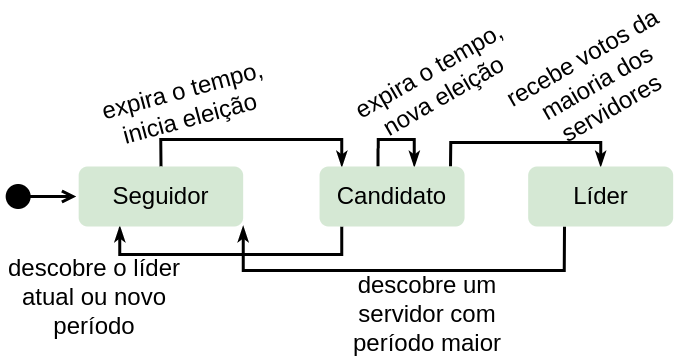
\includegraphics[width=0.75\linewidth]{raft-states.drawio.png}
\label{fig:raft}
{\flushleft Fonte - Adaptado de \cite{raft}}
\end{figure}

A Figura \ref{fig:raft} ilustra os estados de cada nó participante e as possíveis transições. Os seguidores reagem às propostas do líder. Se os candidatos não recebem mais sinais do líder, elege-se um novo líder dentre os candidatos. Se algum candidato estiver no estado de seguidor, este deve poder votar por propostas que chegam ou votar para a eleição de novos líderes. É responsabilidade do líder fazer a replicação dos \textit{logs}. Deve haver apenas 1 líder por termo. O líder é responsável pela replicação de \textit{logs}.

\subsection{Kubernetes}

Kubernetes é uma ferramenta de orquestração de contêineres inicialmente desenvolvida por engenheiros da Google. Kubernetes providencia primitivas tais como: Nodes, Services, Pods, Deployment, Job, Secret, ReplicaSet, StatefulSet, Volume, dentre outras, para que desenvolvedores possam definir Clusters. Kubernetes resolve problemas de estabelecimento de rede entre as máquinas que compõe o Cluster, sejam elas físicas ou virtuais. Kubernetes também resolve problema de replicação de serviços, todavia não garante que os dados das réplicas serão replicados de maneira consistente \cite{kubernetes/docs/2022}. Quando se trata de sistemas com replicação, busca-se uma infraestrutura robusta que permite que cada réplica possa ter seus recursos garantidos \cite{Stubbs2015DistributedSO}, baseado em métricas e tolerante a falhas \cite{vayghan2021kubernetes}.

\section{Hermes} \label{sec:hermes}

O \textit{Hermes} \cite{renan2021hermes} foi programado em linguagem Go. O autor utilizou Kubernetes e Docker para criar o sistema de interceptação, pois cada instância do serviço sendo replicado tem uma outra instância do Hermes à frente, interceptando as requisições. Uma vez interceptadas, as mensagens são submetidas ao protocolo de consenso, para ordenação das mensagens. O \textit{Hermes} utiliza o algoritmo Raft para realizar a ordenação.

% \subsection{COMO OBTIVERAM RESULTADOS (ALTO NÍVEL)}

A avaliação da ferramenta aconteceu através de experimentação no Emulab \cite{emulab-10.1145/844128.844152}, um ambiente para criação de uma rede física de máquinas. O provisionamento do ambiente foi automatizado com a ferramenta Ansible. Os cenários básicos de avaliação foram: sem replicação, replicação à nível de aplicação e replicação no interceptador.

\section{Emulab}

A plataforma Emulab \cite{emulab-10.1145/844128.844152} é um \textit{testbed}, um ambiente de experimentação real. Nesta plataforma é possível criar experimentos, onde o Emulab irá criar a rede de computadores pronta para começar a executar computação paralela.

\section{Trabalhos Correlatos}

\subsection{A Kubernetes controller for managing the availability of elastic microservice based stateful applications}

Segundo \cite{vayghan2021kubernetes} a arquitetura de microsserviços vêm ganhando muita popularidade. A arquitetura de microsserviços faz a junção de módulos fracamente acoplados, que podem ser escalados independentemente. Esse trabalho avalia o uso de microsserviços em contêineres orquestrados por Kubernetes, mas o Kubernetes recebeu um incremento de software que visa controlar os estados de alta disponibilidade dos contêineres. Nesse trabalho de \cite{vayghan2021kubernetes} foram identificados arquiteturas para implantar aplicações em microsserviços com Kubernetes. Esse trabalho também realizou experimentações com o Kubernetes da perspectiva de sua capacidade de disponibilidade. Os resultados dos experimentos mostraram que as ações de reparo do Kubernetes não puderam satisfazer alguns limites de alta disponibilidade, avaliados. Em outros casos o Kubernetes não pode garantir recuperação do serviço. Os autores propuseram um controlador de estados de alta disponibilidade integrado ao Kubernetes, que permite replicação de estados de aplicação e redirecionamento automático de serviço. As avaliações foram feitas sob as perspectivas de disponibilidade e escalabilidade. Os resultados das investigações mostram que a solução pode melhorar o tempo de recuperação de aplicações \textit{stateful} baseadas em microsserviços, em 50\%.

\subsection{\textit{Incorporating the Raft consensus protocol in containers managed by Kubernetes: an evaluation}}

O trabalho de \cite{netto2020incorporating} visa implementar uma solução de replicação por máquinas de estados usando Raft como algoritmo de consenso. A sua solução foi construída no topo do orquestrador de contêineres Kubernetes. Esse trabalho optou por utilizar o Raft ao invés do Paxos, pela didática e praticidade.

Para desenvolver a solução os autores escolheram o algoritmo Raft e buscaram um código livre e aberto em linguagem Go. O código foi inserido no contexto de orquestração de contêineres. Esse trabalho visou utilizar o banco de dados Etcd. Os autores estenderam uma biblioteca para poder acrescentar funcionalidades personalizadas ao Kubernetes. Foram adicionados:

\begin{itemize}
\item Mecanismo próprio de descoberta de réplicas usando API do Kubernetes.
\item Aceitação de requisições por qualquer réplica.
\end{itemize}

\subsection{\textit{Implementação de um interceptador para ordenação de mensagens em arquiteturas baseadas em microsserviços}}

\cite{renan2021hermes} propôs uma arquitetura em ambientes de microsserviços para o desacoplamento da lógica de ordenação de mensagens. Um dos objetivos era manter consistência forte em um sistema replicado. Para isto, implementou-se replicação por máquinas de estados usando intercepção de mensagens que chegam ao serviço Hermes. O serviço, baseia-se em padrões de projeto voltados para arquiteturas de microsserviços. O código criado por \cite{renan2021hermes} provê interfaces que uma vez implementadas possibilitam que outros protocolos de consenso sejam incluídos, e também outros protocolos de comunicação.

\section{Desenvolvimento} \label{sec:des}

Foram realizadas mudanças no desenvolvimento na forma de comunicação do Hermes. A mudança permite, o Hermes aceitar requisições HTTP de maneira genérica. Para isso, foi necessário implementar a interface \textit{Communicator}. Durante o desenvolvimento, foi criado um projeto do Hermes com: Docker, Docker Compose e Delve\footnote{Delve é um depurador de código linguagem Go.}. A implementação tomou o nome de \textit{HttpCommunicator}, seguindo o padrão de nomes previamente implementado.

A classe \textit{HTTPCommunicator} está localizada em \textit{pkg/communication/http.go}. Para implementar a \textit{HTTPCommunicator} foram usadas as bibliotecas \textit{net/http, bufio, bytes, io/ioutil}, dentre outras. A necessidade de estender as bibliotecas de conversão de bytes foi para poder transformar a requisição em bytes e enviar ao \textit{handler} ordenador de mensagens. Uma vez que o Hermes devolve a mensagem ordenada para o \textit{HTTPCommunicator}, é preciso transformar a mensagem de bytes para uma Requisição executável pela biblioteca \textit{net/http}.

\begin{minipage}{\textwidth}
\begin{center}
\lstinputlisting[language=Go, numbers=left, firstnumber=1, numberstyle=\scriptsize\color{black}, caption={Código na versão resumida do HttpCommunicator}, label={lst:codigo-httpcomm}]{http.go}
\end{center}
\end{minipage}

O Algoritmo \ref{lst:codigo-httpcomm} pode ser entendido da seguinte forma: A linha 14 converte a requisição {HTTP} para \textit{bytes} (código omitido). A linha 16 faz com que o Hermes acione o mecanismo de ordenação de mensagens, passando os bytes para serem ordenados. Depois que os bytes foram ordenados eles vão eventualmente retornar para o \textit{Deliver} para serem entregues para o servidor da aplicação, para isso a linha 2 converte os bytes em requisição (código omitido). Com a requisição convertida, altera-se o \textit{HOST} alvo nas linhas 4-6. A variável \textit{RequestURI} na linha 8 está sendo transformada para \textit{string} vazia, pois a biblioteca de \textit{net/http} proíbe que a mesma requisição seja usada, desta maneira a biblioteca aceita executar a requisição. Finalmente, a variável \textit{URI.Scheme} na linha 9 está sendo preenchida com o protocolo {HTTP}. O código completo pode ser encontrado em \url{https://github.com/tonussi/hermes}.

\section{Resultados} \label{sec:res}

O Emulab foi a plataforma utilizada para experimentações e obtenção de resultados. Nesta plataforma foram alocadas 3 máquinas para os servidores de ordenação de mensagens e 2 máquinas para os geradores de carga. A máquina usada para os experimentos foi a d710. A especificações são as seguintes: marca Dell Poweredge R710, processador 2.4 GHz 64-bit Quad Core Xeon E5530 "Nehalem", cache de 8 MB L3, memória de 12 GB 1066 MHz DDR2 RAM (6 módulos de 2GB), discos rígidos de 500GB e 250GB 7200 rpm SATA.


Os experimentos mostram as vazões médias em requisições por segundo no eixo $x$ e as latências dadas pelo nonagésimo percentil em milissegundos no eixo $y$. A seguir serão apresentados os gráficos comparativos dos experimentos.

\begin{figure}[htb!]
\centering
\caption{Requisição GET invocando a função \textit{get\_line} no servidor}
\includesvg[width=\linewidth]{get-line.svg}
\label{fig:get-line}
\end{figure}

A Figura \ref{fig:get-line} mostra que nos pontos de 8-20 req/s o Hermes estava com aproximadamente 7 ms de latência, já no intervalo de 20 até 40 req/s o Hermes obteve latências próximos de 144 ms. O cenário sem replicação obteve latências em torno de 5 ms entre o período de 10 até aproximadamente 68 req/s. O Hermes apresentou consistência até 30 req/s, porém em aproximadamente 60 req/s ocorreu uma estagnação da vazão e crescimento da latência, o mesmo comportamento aconteceu para o sistema sem replicação, porém perto de 80 requisições por segundo. O cenário de 100\% requisições GET precisa que exista dados pre-populado com \textit{strings} de 128-bytes para que seja possível obter as linhas, 1000 linhas são pre-populadas e talvez isso faça que com o sistema Hermes obtenha vazão até 60 req/s e então estagne.

\begin{figure}[htb!]
\centering
\caption{Requisição GET/POST invocando as funções \textit{get\_line} e \textit{append\_line} no servidor}
\includesvg[width=\linewidth]{get-append-line.svg}
\label{fig:get-append-line}
\end{figure}

A Figura \ref{fig:get-append-line} mostra que para o caso de 50\% GET e 50\% POST faz com que a vazão estagne antes de 60\%. Isto pode significar que no caso de 50\% GET 50\% POST é preciso preencher dados para haver vazão. Notar que em todos os cenários há pre-população de dados. O ponto de saturação do Hermes pode ser observado em aproximadamente 40 req/s, já o ponto de saturação no cenário sem replicação pode ser observado em aproximadamente 80 req/s.

As latências do Hermes se mantiveram aproximadamente 7 ms entre 8 até 20 req/s e a partir de 30 req/s a latência cresceu até aproximadamente 170 ms. Em 60 req/s a latência subiu e estagnou no ponto de 60 req/s. O cenário sem replicação obteve latências de aproximadamente 5 ms desde 10 req/s até aproximadamente 70 req/s e estagnou crescendo latência e obtendo vazões entre 70 e 80 req/s. O ponto de saturação do Hermes pode ser observado em aproximadamente 35 req/s, já o ponto de saturação no cenário sem replicação pode ser observado em aproximadamente 68 req/s.

\pagebreak

\begin{figure}[htb!]
\centering
\caption{Requisição POST invocando a função \textit{append\_line} no servidor}
\includesvg[width=\linewidth]{append-line.svg}
\label{fig:append-line}
\end{figure}

A Figura \ref{fig:append-line} mostra que o Hermes obteve latências de aproximadamente 7 ms entre o período de 10 até aproximadamente 70 req/s. Entre 70 e 80 req/s o Hermes apresentou estagnação da vazão enquanto a latência aumentou para 225 ms. O cenário sem replicação obteve latências de aproximadamente 5 ms entre 10 até aproximadamente 80 req/s. Em 80 req/s começou a estagnar a vazão de requisições, subindo a latência até aproximadamente 200 ms. O ponto de saturação do Hermes pode ser observado em aproximadamente 68 req/s, já o ponto de saturação no cenário sem replicação pode ser observado em aproximadamente 78 req/s.

Em geral, há sobrecarga ao usar o Hermes. A sobrecarga foi baixa no cenário 100\% \textit{POST}, que é um comportamento \textit{append-only}, onde apenas se adiciona uma linha no fim do arquivo de (\textit{log}). O custo da latência em ms fica bastante elevado com a presença de comandos \textit{GET}.

\section{Conclusão}

O presente artigo apresentou uma forma de comunicação via HTTP para o interceptador e ordenador de mensagens, Hermes. Esta forma de comunicação permite que aplicações que trabalham com HTTP, possam ser replicadas. Os desenvolvedores podem focar na lógica de negócio da sua aplicação ou {API}, sem se preocuparem com detalhes de ordenação. Este trabalho é também, um estudo sobre: a arquitetura geral do interceptador Hermes; técnicas de ordenação, orquestradores de contêineres, algoritmos de consenso e tópicos relacionados.

Os experimentos com o ordenador Hermes mostraram latências mais altas em relação ao sistema sem replicação. As leituras em arquivo de uma linha aleatória a cada requisição \textit{GET} fazem com que os gráficos mostrem que o servidor consegue responder em baixas latências até determinada implicação de carga, mas sobe abruptamente em certo ponto. Durante os experimentos, foram feitas diversas tentativas de coleta de pontos e foram criados várias configurações de experimentação, porém os resultados sempre estavam culminando para algo parecido. Contudo, a escrita em arquivo pela requisição POST se demostrou mais previsível nos gráficos, aparentando uma subido gradual da latência enquanto a vazão estagnava.

\bibliographystyle{sbc}
\bibliography{sbc-template}

\end{document}
